\chapter{Asynchronous Concurrency}

In the previous chapters, we explored how traditional multithreading allows us to perform multiple tasks simultaneously. Multithreading is highly effective for CPU-bound workloads, where calculations can be distributed across multiple physical cores to reduce total execution time. However, when dealing with I/O-bound workloads---such as web servers managing thousands of concurrent requests, or systems performing extensive file system searches---spawning a dedicated thread for every operation quickly becomes inefficient.

The professor emphasizes a fundamental distinction: \textit{concurrency} is about dealing with multiple tasks overlapping in time, while \textit{parallelism} is about executing multiple tasks exactly at the same time. Asynchronous programming in Rust is a powerful tool to achieve massive concurrency, allowing a single thread to manage thousands of I/O operations without blocking.

In this chapter, we will introduce asynchronous concurrency in Rust. We will explore how it fundamentally differs from thread-based concurrency, how Rust implements it under the hood using state machines and the \texttt{Future} trait, and how to build robust concurrent applications using the Tokio runtime, tasks, asynchronous mutexes, and channels.

\section{The Limits of Standard Threads}

When a program performs an I/O operation, such as reading from a disk or a network socket, the operating system blocks the requesting thread until the data is ready. If we have thousands of concurrent requests, a traditional multi-threaded approach would require spawning thousands of threads. 

This approach has severe drawbacks:
\begin{itemize}
    \item \textbf{Memory Overhead:} Every standard thread requires a pre-allocated stack (often 1-2 MB). As the professor noted, a typical enterprise system might start with 500 threads, immediately consuming 500 MB of RAM just for idle stacks! Having 10,000 threads means allocating gigabytes of memory just for the stacks, even if the threads spend 99.9\% of their time waiting for data.
    \item \textbf{Context Switch Cost:} The OS preemptive scheduler must continuously switch context between threads. Context switching involves saving registers, invalidating caches, and updating the Translation Lookaside Buffer (TLB), taking microseconds per switch. With thousands of threads, these overheads sum up to significant delays.
\end{itemize}

\begin{insightbox}[The True Cost of I/O: The Heartbeat Analogy and the Bakery]
To understand why waiting for I/O in standard threads is so devastating to performance, the professor provides a vivid analogy mapping CPU clock cycles to human time. If a single CPU cycle is equivalent to one human heartbeat (about 1 second):
\begin{itemize}
    \item Accessing L1 cache takes 1-2 heartbeats.
    \item Accessing L2/L3 cache takes around 15 heartbeats.
    \item Accessing main memory (RAM) takes about 4 minutes.
    \item Reading from a generic SSD takes from 1.5 to 4 days.
    \item Sending a network packet across the internet is equivalent to waiting 5 years!
\end{itemize}
When a thread blocks on network I/O, the CPU is essentially forced to wait "years" in relative time. To mitigate these memory delays, modern CPUs rely heavily on caches. The professor compares this to a \textit{Panetteria} (bakery): a baker doesn't buy ingredients for one sandwich at a time. They fetch in bulk (like the CPU fetching a whole cache line) because it's statistically probable that adjacent data will be needed soon (spatial locality). By using small, fast stores (L1) fed by medium stores (L2) and large stores (L3), the CPU minimizes the catastrophic "4-minute" RAM penalty.
\end{insightbox}

\begin{insightbox}[Parallel Execution vs. Parallel Waiting]
Use standard threads to \textit{compute} in parallel (CPU-bound tasks). Use asynchronous programming to \textit{wait} in parallel (I/O-bound tasks). Asynchronous concurrency allows a single thread to manage thousands of concurrent I/O operations without blocking.
\end{insightbox}

\section{The Rust Async Model: Cooperative Scheduling}

Instead of relying on the operating system's preemptive scheduler to pause threads, asynchronous Rust uses a \textbf{cooperative scheduling} approach at the application level. This concept is closely related to what are historically known as \textit{green threads} or \textit{fibers}. While native threads are scheduled preemptively by the OS, green threads yield control voluntarily. In Rust, this is achieved via the async runtime, which manages these lightweight tasks without the heavy OS context switches.

\subsection{The \texttt{Future} Trait and State Machines}
When you define a function with the \texttt{async} keyword, the compiler transforms the function body into a state machine that implements the \texttt{Future} trait. Calling an \texttt{async} function does not immediately execute its body. Instead, it instantly returns an inert \texttt{Future} object.

\begin{lstlisting}[language=Rust]
async fn fetch_data() -> String {
    // This code does not run immediately!
    "Data loaded".to_string()
}

// In another function:
let my_future = fetch_data(); // Returns a Future, execution has not started.
\end{lstlisting}

To actually execute a \texttt{Future}, it must be \textit{polled}. The \texttt{Future} trait defines a \texttt{poll} method that returns either:
\begin{itemize}
    \item \texttt{Poll::Pending}: The operation is not yet complete. The future yields control back to the executor.
    \item \texttt{Poll::Ready(value)}: The operation has finished, returning the result.
\end{itemize}

When you use the \texttt{.await} keyword on a future, you instruct the system to suspend the current asynchronous task if the future returns \texttt{Pending}.

\begin{notebox}
The \texttt{.await} syntax marks explicit \textbf{suspension points}. It tells the executor: ``If this value isn't ready yet, park this task and go execute another one. Wake me up when the data is ready.'' This is the core of cooperative scheduling.
\end{notebox}

\subsection{The Executor and the Waker}
Because futures are inert, an \textbf{executor} (often part of a runtime like Tokio) is responsible for polling them in a loop. When a future returns \texttt{Pending}, it registers a \texttt{Waker} with the underlying I/O subsystem. Once the hardware or operating system signals that the data is ready, the \texttt{Waker} notifies the executor, which then re-polls the future. This mechanism ensures that the CPU does not waste cycles busy-polling empty queues.

\section{Building Async Programs with Tokio}

Rust's standard library provides the \texttt{Future} trait and the basic building blocks for asynchronous programming, but it intentionally does not include an executor. The most widely used asynchronous runtime in the Rust ecosystem is \textbf{Tokio}.

To use Tokio, you must include it in your \texttt{Cargo.toml} with the \texttt{full} feature flag, and annotate your main function.

\begin{lstlisting}[language=Rust]
#[tokio::main]
async fn main() {
    println!("Hello from the async world!");
}
\end{lstlisting}
The \texttt{\#[tokio::main]} macro rewrites your \texttt{main} function to initialize the Tokio runtime (allocating worker threads and message queues) and then executes the asynchronous body inside that runtime.

\subsection{Spawning Independent Tasks: \texttt{tokio::spawn}}
When you write \texttt{.await}, you are creating a sequential dependency: the current task cannot proceed until the awaited future completes. If you want to run independent asynchronous activities concurrently, you use \texttt{tokio::spawn}.

\begin{lstlisting}[language=Rust]
use tokio::task;

#[tokio::main]
async fn main() {
    // Spawn an independent background task
    let handle = tokio::spawn(async {
        // This block runs concurrently
        tokio::time::sleep(std::time::Duration::from_secs(1)).await;
        "Task finished"
    });

    // The main task continues immediately
    println!("Doing other work...");

    // Optionally await the spawned task's JoinHandle to get its result
    let result = handle.await.unwrap();
    println!("Result: {}", result);
}
\end{lstlisting}

\textbf{Deep Memory Model Analysis:}
In this snippet, \texttt{tokio::spawn} creates a new asynchronous task. The \texttt{async} block generates an anonymous state machine structure. Since the \texttt{async} block takes ownership of no variables here, the state machine size is very small and is allocated on the heap by the Tokio runtime to ensure its lifetime is independent of the current function frame. The \texttt{handle} returned is a \texttt{JoinHandle}, which is a lightweight struct placed on the current task's stack. When \texttt{.await} is called on the handle, it checks the heap-allocated state of the spawned task. If we were capturing variables, they would be moved (ownership transfer) into the heap-allocated state machine because the task must be \texttt{'static} and \texttt{Send}. There is no borrowing (\texttt{\&}) allowed from the local stack since the spawned task might outlive the stack frame or execute on a different OS thread.


\begin{warningbox}
Futures spawned with \texttt{tokio::spawn} must be \texttt{Send} and \texttt{'static}. Because Tokio's default executor is multi-threaded, tasks can yield on one thread and be resumed on another. Therefore, any data captured by the async block must be safely transferable across thread boundaries (\texttt{Send}) and cannot contain references to local variables that might go out of scope (\texttt{'static}).
\end{warningbox}

\begin{examprioritybox}[The \texttt{Send} and \texttt{'static} Constraints]
The professor heavily emphasizes the requirements for background tasks: they must own their data (\texttt{'static}) and be safe to move across threads (\texttt{Send}). Forgetting to \texttt{move} variables or using \texttt{Rc} inside a spawned task will immediately cause a compilation error.
\textbf{Common Pitfall:} Attempting to borrow local variables inside \texttt{tokio::spawn} or passing non-thread-safe types like \texttt{Rc<T>}.
\textbf{Expected Mastery Level:} High. You must fluently explain why the borrow checker rejects non-\texttt{'static} references in tasks and how to fix it (e.g., using \texttt{Arc} or passing by value).
\end{examprioritybox}


\subsection{Combining Futures: \texttt{join!} and \texttt{select!}}
Sometimes you need to coordinate multiple futures without spawning completely independent tasks:
\begin{itemize}
    \item \textbf{\texttt{tokio::join!}}: Runs multiple futures concurrently on the \textit{same task} and waits for all of them to complete. The total time taken is approximately the duration of the longest future.
    \item \textbf{\texttt{tokio::select!}}: Runs multiple futures concurrently, but waits only for the \textit{first} one to complete. Once a future resolves, the others are immediately cancelled (aborted). This is highly useful for implementing timeouts or listening for cancellation signals.
\end{itemize}

\subsection{Avoiding Executor Starvation}
Because Tokio's scheduler is cooperative, tasks must yield control voluntarily via \texttt{.await}. If you insert a long CPU-bound loop or a blocking standard library call (like \texttt{std::thread::sleep}) inside an \texttt{async} function, you will block the underlying worker thread. This prevents other asynchronous tasks from being executed!

Always use asynchronous alternatives like \texttt{tokio::time::sleep}. For unavoidable, heavy CPU-bound computations, offload the work using \texttt{tokio::task::spawn\_blocking}, which runs the closure on a dedicated thread pool specifically designed for blocking operations.

\section{Shared State and Synchronization}

Just like in standard multithreading, concurrent tasks often need to share data. While passing ownership or using channels is preferred, sometimes a shared state is necessary. 

The professor uses a practical analogy to explain shared state: imagine preparing your lunch and leaving it in the shared office refrigerator. In a sequential world (living alone), you can safely assume your lunch will be exactly as you left it. But in a concurrent world, another thread (or colleague) might modify it or eat it! The solution is putting a padlock (\textit{catenaccio}) on the refrigerator. This lock is exactly what a \texttt{Mutex} provides, ensuring mutually exclusive access.

However, in an async environment, you must be careful. If you wrap data in an \texttt{Arc<std::sync::Mutex>}, blocking the mutex will block the entire worker thread, stalling the executor. To solve this, Tokio provides \texttt{tokio::sync::Mutex}.

\begin{lstlisting}[language=Rust]
use std::sync::Arc;
use tokio::sync::Mutex;

#[tokio::main]
async fn main() {
    let counter = Arc::new(Mutex::new(0));
    let mut handles = vec![];

    for _ in 0..10 {
        let counter_clone = Arc::clone(&counter);
        let handle = tokio::spawn(async move {
            // lock().await suspends the task if the lock is held by someone else,
            // allowing the thread to execute other tasks in the meantime!
            let mut num = counter_clone.lock().await;
            *num += 1;
        });
        handles.push(handle);
    }

    for handle in handles {
        handle.await.unwrap();
    }

    println!("Final count: {}", *counter.lock().await);
}
\end{lstlisting}

\subsection{Synchronous Coordination: Mutex and Condvar (Bounded Buffer)}

While Tokio provides asynchronous synchronization, traditional OS threads rely on \texttt{std::sync::Mutex} and \texttt{std::sync::Condvar} to coordinate complex state changes. The professor illustrates this by building a \textbf{Bounded Buffer}---a thread-safe, fixed-capacity FIFO queue where producers must wait if it's full, and consumers must wait if it's empty.

% AI-IMAGE-REQUEST: A diagram showing a Bounded Buffer queue with a Producer thread waiting on a full condition, and a Consumer thread taking elements out.
\begin{figure}[h]
    \centering
    \includegraphics[width=0.8\textwidth]{images/bounded_buffer.png}
    \caption{A thread-safe Bounded Buffer using Mutex and Condvar.}
    \label{fig:bounded_buffer}
\end{figure}

To implement this, we encapsulate a \texttt{VecDeque} and a boolean \texttt{closed} flag inside a \textit{single} \texttt{Mutex}, paired with a \texttt{Condvar}:

\begin{lstlisting}[language=Rust]
use std::collections::VecDeque;
use std::sync::{Mutex, Condvar};

pub struct BoundedBuffer<T> {
    // Both the queue and the 'closed' flag MUST be in the same Mutex
    data: Mutex<(VecDeque<T>, bool)>,
    cv: Condvar,
    capacity: usize,
}

impl<T: Send> BoundedBuffer<T> {
    pub fn new(capacity: usize) -> Self {
        BoundedBuffer {
            data: Mutex::new((VecDeque::new(), true)), // true = open
            cv: Condvar::new(),
            capacity,
        }
    }

    pub fn push(&self, item: T) -> bool {
        let mut guard = self.cv.wait_while(self.data.lock().unwrap(), |(q, is_open)| {
            q.len() >= self.capacity && *is_open
        }).unwrap();

        if !guard.1 { return false; } // If closed, abort push

        guard.0.push_back(item);
        
        // OPTIMIZATION: Drop the lock BEFORE notifying, so the woken thread 
        // doesn't immediately block trying to acquire the Mutex.
        drop(guard); 
        self.cv.notify_all();
        true
    }

    pub fn pop(&self) -> Option<T> {
        let mut guard = self.cv.wait_while(self.data.lock().unwrap(), |(q, is_open)| {
            q.is_empty() && *is_open
        }).unwrap();

        if guard.0.is_empty() {
            return None; // Woke up because it was closed and empty
        }

        let item = guard.0.pop_front().unwrap();
        drop(guard);
        self.cv.notify_all();
        Some(item)
    }
}
\end{lstlisting}

\begin{insightbox}[Condvar Best Practices]
\textbf{1. All state in one Mutex:} A common mistake is using two Mutexes for two variables. The Condvar can only unlock \textit{one} Mutex while sleeping. All related state (like the queue and the closed flag) must be in the \textit{same} Mutex tuple.

\textbf{2. \texttt{wait\_while}:} Always use \texttt{wait\_while} (or a loop) to wait. This protects against "spurious wakeups" and ensures the condition is evaluated securely.

\textbf{3. Drop before Notify:} By manually dropping the Mutex guard (\texttt{drop(guard);}) before calling \texttt{notify\_all()}, we prevent a performance penalty where the woken thread instantly goes back to sleep because the notifier still holds the lock.
\end{insightbox}

\textbf{Deep Memory Model Analysis:}
Here, \texttt{Arc::new(Mutex::new(0))} allocates both the reference counter and the Mutex state on the heap. The variable \texttt{counter} itself is a smart pointer on the main task's stack. Inside the loop, \texttt{Arc::clone(\&counter)} increments the atomic reference count and creates a new \texttt{Arc} pointer (\texttt{counter\_clone}) on the stack. The \texttt{async move} closure takes ownership of \texttt{counter\_clone}, moving it into the task's heap-allocated state machine. When \texttt{lock().await} yields a \texttt{MutexGuard}, this guard is placed into the state machine's state so it can be held across suspension points. Once the lock is acquired, the guard provides a mutable reference (\texttt{\&mut i32}) to the heap-allocated integer, safely avoiding data races. Finally, the guard is dropped at the end of the block, releasing the Mutex lock.

\textbf{Practical Mastery Focus: When and Why to Use \texttt{tokio::sync::Mutex}}
Use \texttt{tokio::sync::Mutex} \textit{only} when you need to hold the lock across an \texttt{.await} suspension point. If your critical section is brief, contains no asynchronous operations, and merely updates a quick value (like a counter), use the standard \texttt{std::sync::Mutex}. The standard mutex is much faster and less memory-intensive for purely synchronous state updates.


\begin{exambox}[Async Mutex vs. Standard Mutex]
Exam questions frequently ask why \texttt{tokio::sync::Mutex} is needed. The key distinction is that \texttt{tokio::sync::Mutex::lock()} is an asynchronous method (\texttt{.await}). If the mutex is already locked, it suspends the \textit{task} rather than blocking the OS \textit{thread}. This frees the executor's worker thread to poll other pending tasks.
\end{exambox}

\begin{warningbox}[Hardware Realities: Atomicity, Visibility, and Ordering]
The existence of CPU caches and instruction reordering introduces three critical problems in multithreading that are purely \textit{hardware facts}, totally independent of the programming language:
\begin{enumerate}
    \item \textbf{Atomicity:} An operation like \texttt{A += 1} might require multiple assembly instructions (fetch, increment, store). A thread might be interrupted halfway, leaving corrupted data.
    \item \textbf{Visibility:} A core writes a value to its local L1 cache. Unless explicitly flushed, other cores reading from their own L1 caches will not see this update.
    \item \textbf{Ordering:} Concurrency fundamentally introduces non-determinism. As the professor's "red shirt" analogy highlights: if you tell a friend "when I put on my red shirt, I'm ready to go", a highly optimized system might reorder your actions, putting the red shirt on you \textit{before} you are actually ready, simply because it sees no local data dependency!
\end{enumerate}
To solve these, processors provide specific hardware instructions called \textit{Memory Barriers} or \textit{Fences} (e.g., \texttt{FENCE} on x86, \texttt{Barrier} on ARM) that force cache synchronization. High-level synchronization primitives automatically use these barriers under the hood.
\end{warningbox}

\begin{examprioritybox}[Execution Non-Determinism and Memory Visibility]
The professor frequently emphasizes that the main difficulties in concurrency arise from non-determinism, atomicity, visibility, and ordering. Memory barriers are required to prevent caches and CPUs from reordering instructions in ways that violate logical sequencing.
\textbf{Common Pitfall:} Assuming sequential execution order is preserved globally across multiple threads without explicit synchronization.
\textbf{Expected Mastery Level:} Very High. You must recognize that synchronization isn't just about mutual exclusion; it's also about enforcing memory visibility across thread caches.
\end{examprioritybox}


\section{Message Passing: Channels in Tokio}

To coordinate tasks without shared state, Tokio offers a rich set of asynchronous channels, conceptually expanding on the standard library's channels. The architecture and relationships of these channels can be visualized as follows:

\begin{figure}[h]
    \centering
    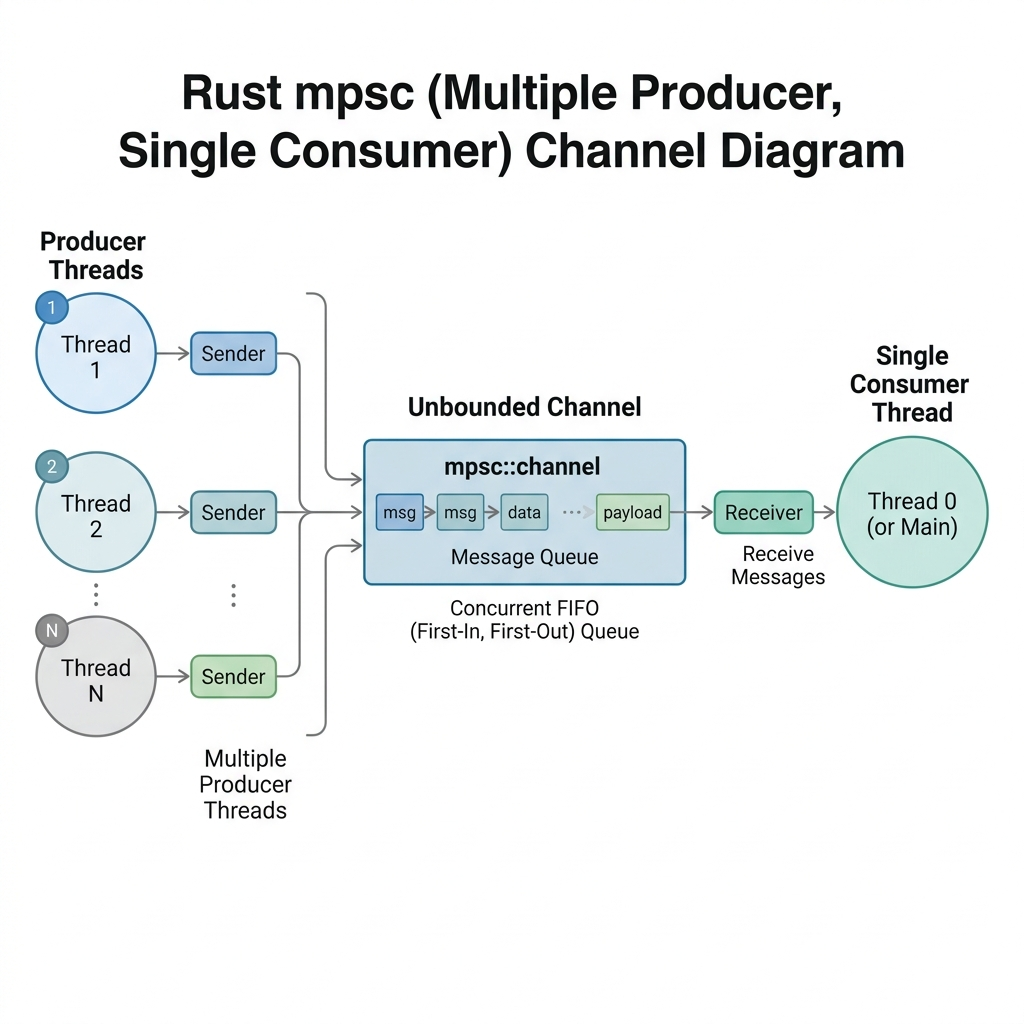
\includegraphics[width=0.8\textwidth]{images/mpsc_channel.png}
    \caption{Overview of asynchronous message passing patterns.}
    \label{fig:async_channels}
\end{figure}

Tokio provides four main types of channels:
\begin{enumerate}
    \item \textbf{oneshot}: A single producer sends exactly one message to a single consumer. Ideal for sending a specific result back to an awaiting task.
    \item \textbf{mpsc} (Multiple Producer, Single Consumer): Bounded channels designed for high-throughput streaming of messages.
    \item \textbf{broadcast}: Multiple producers can broadcast messages to multiple consumers. Every receiver gets a copy of the message.
    \item \textbf{watch}: Multiple consumers monitor a single value. When the producer updates the value, consumers are notified of the change.
\end{enumerate}

\subsection{Backpressure and the MPSC Channel}

The most commonly used channel is the \texttt{mpsc} channel. Unlike the unbounded channels in the standard library, Tokio's \texttt{mpsc} channels are inherently \textbf{bounded}. You must specify a capacity when creating them.

\begin{lstlisting}[language=Rust]
use tokio::sync::mpsc;

#[tokio::main]
async fn main() {
    // Create an MPSC channel with a capacity of 10 messages
    let (tx, mut rx) = mpsc::channel(10);

    tokio::spawn(async move {
        for i in 0..20 {
            // If the channel is full, send().await suspends this task!
            if tx.send(i).await.is_err() {
                println!("Receiver dropped!");
                return;
            }
        }
    });

    // Simulate a slow consumer
    while let Some(msg) = rx.recv().await {
        println!("Received: {}", msg);
        tokio::time::sleep(std::time::Duration::from_millis(100)).await;
    }
}
\end{lstlisting}

\textbf{Deep Memory Model Analysis:}
The \texttt{mpsc::channel(10)} call allocates the channel's shared state (a queue and wait lists) on the heap. It returns \texttt{tx} (a \texttt{Sender}) and \texttt{rx} (a \texttt{Receiver}) to the main task's stack. The \texttt{async move} block transfers ownership of the \texttt{Sender} to the spawned task's heap-allocated state. When \texttt{tx.send(i).await} is called, the value \texttt{i} (allocated initially on the task's stack) is copied/moved into the heap queue. If the queue is full (size $\ge$ 10), the future returned by \texttt{send} returns \texttt{Poll::Pending}, parking the task and saving its state. When the main task consumes a message via \texttt{rx.recv().await}, the message is moved from the heap queue back to the main task's stack (\texttt{msg}), and the channel wakes the parked producer task so it can resume sending.


This bounding mechanism introduces \textbf{backpressure} into the system. If the producer is generating messages faster than the consumer can process them, the channel will fill up. Once the channel reaches its capacity of 10, the next \texttt{tx.send(val).await} call will return \texttt{Poll::Pending}, suspending the producer task. 

Backpressure is a critical property of robust distributed systems: it prevents a fast producer from exhausting the system's memory by queuing an infinite number of messages, forcing the producer to slow down and match the consumer's pace.

\subsection{Common Channel Patterns}

The professor highlights three major concurrent architectural patterns that are easily implemented using channels (whether standard, \texttt{crossbeam}, or Tokio):

\begin{enumerate}
    \item \textbf{Fan-In / Fan-Out:} A single producer generates tasks (e.g., parsing PDFs). Multiple worker threads compete to pull messages from the same channel (Fan-Out). The first available worker grabs the task, processes it, and sends the result to an output channel collected by a single consumer (Fan-In). This maximizes CPU usage but \textit{does not guarantee the order} of results.
    \item \textbf{Pipeline:} Data flows sequentially through discrete stages (Producer $\rightarrow$ Stage 1 $\rightarrow$ Stage 2 $\rightarrow$ Consumer). Unlike Fan-Out, a pipeline maintains the exact order of the data. It is highly effective when individual processing steps are heavy and can be offloaded to separate threads.
    \item \textbf{Thread Pool (Producer-Consumer):} A specialized Fan-Out where the channel doesn't transmit raw data, but rather executable closures (\texttt{Box<dyn FnOnce() + Send>}). The worker threads act as generic executors that simply pop a function from the channel and run it.
\end{enumerate}

% AI-IMAGE-REQUEST: Diagram illustrating Fan-In/Fan-Out and Pipeline architectures with channels connecting producer and consumer threads.
\begin{figure}[h]
    \centering
    \includegraphics[width=0.8\textwidth]{images/channel_patterns.png}
    \caption{Fan-In/Fan-Out and Pipeline channel patterns.}
    \label{fig:channel_patterns}
\end{figure}

\section{Choosing Between Shared State and Channels}

At the end of the concurrency lecture, the professor provides a definitive checklist for deciding how to synchronize threads:

\begin{enumerate}
    \item \textbf{Is there a simple channel-based solution?} If yes, use it. Channels are generally safer and less prone to subtle logic errors. 
    \item \textbf{Do you need to wait for a specific event or condition?} Use a \texttt{Condvar} (or async equivalent). Channels can signal completion, but \texttt{Condvar} allows waiting for complex, multi-variable state changes.
    \item \textbf{Do you have complex interlocking state?} Use \texttt{Mutex} and shared state. It is the most general solution, but requires the highest discipline to avoid bugs.
\end{enumerate}

\begin{warningbox}[The Three Deadlocks of Shared State]
When writing complex shared state, always audit for:
\begin{itemize}
    \item \textbf{Deadlock:} Thread A waits for Thread B, and Thread B waits for Thread A. Execution halts.
    \item \textbf{Livelock:} Threads continuously yield to each other out of "politeness", burning CPU cycles but making no forward progress.
    \item \textbf{Starvation:} A low-priority thread is perpetually bypassed by faster/higher-priority threads, never acquiring the Mutex.
\end{itemize}
\end{warningbox}

\section{Domande ed Esercizi da Esami Passati}

\begin{exambox}[Domanda: TokenManager]
\textbf{Testo:} Un applicativo software multithread fa accesso ai servizi di un server remoto, attraverso richieste di tipo HTTP. Tali richieste devono includere un token di sicurezza... Poiché la emissione richiede un tempo apprezzabile, si vuole centralizzare la gestione del token.

\textbf{Soluzione basata sul capitolo:} La gestione centralizzata del token può essere implementata utilizzando un pattern di stato condiviso protetto da \texttt{Mutex} e \texttt{Condvar} (come mostrato nel pattern \texttt{BoundedBuffer}), dove un singolo thread coordina il rinnovo. In alternativa, in un contesto asincrono Tokio, si applica il pattern \textbf{Producer-Consumer} usando canali: un task produttore rinnova il token e lo distribuisce via canale. Per un singolo valore aggiornato e distribuito a più task richiedenti, il testo suggerisce l'uso del canale \textbf{watch}.
\end{exambox}

\begin{exambox}[Domanda: DelayedExecutor]
\textbf{Testo:} La struct \texttt{DelayedExecutor} permette di eseguire funzioni in modo asincrono, dopo un certo intervallo di tempo...

\textbf{Soluzione basata sul capitolo:} Per eseguire un ritardo in modo asincrono senza bloccare l'executor, si usa \texttt{tokio::time::sleep} all'interno di un task generato con \texttt{tokio::spawn} (anziché il bloccante \texttt{std::thread::sleep}). Per l'accodamento dei job, l'architettura sfrutta il pattern architetturale \textbf{Thread Pool (Producer-Consumer)}, accodando chiusure eseguibili (\texttt{Box<dyn FnOnce() + Send>}) in un canale che risveglierà i task in attesa al momento opportuno.
\end{exambox}

\begin{exambox}[Domanda: Aggregatore di misure]
\textbf{Testo:} Un sistema di monitoraggio raccoglie misure di temperatura da più sensori. Le misure vengono raccolte in modo asincrono... Compito del sistema è aggregare le misure ricevute...

\textbf{Soluzione basata sul capitolo:} Questo scenario corrisponde direttamente al pattern \textbf{Fan-In} tramite canali \texttt{mpsc}. Molti thread (sensori) agiscono come \textit{producer} che inviano i dati attraverso il canale concorrente, affidando l'esclusione mutua al meccanismo interno del canale. Un singolo thread consumatore (l'aggregatore) legge i messaggi e calcola le medie, seguendo la regola aurea presentata nel capitolo: "Is there a simple channel-based solution?".
\end{exambox}

\begin{exambox}[Domanda: Race conditions e Thread]
\textbf{Testo:} Si definisca un esempio in cui... si possano evitare raceconditions nel momento in cui i thread debbano accedere in scrittura alla stessa risorsa. Si distingua il caso in cui tale risorsa sia uno scalare e quella in cui sia una struttura più articolata.

\textbf{Soluzione basata sul capitolo:} Per risorse scalari (come un contatore) il capitolo consiglia l'uso di \texttt{std::sync::Mutex} per garantire accesso esclusivo e gestire l'atomicità hardware. Se la risorsa è complessa (es. \texttt{BoundedBuffer}), è necessario combinare \texttt{Mutex} con \texttt{Condvar}, assicurandosi che \textit{tutto} lo stato correlato risieda nello stesso \texttt{Mutex} (evitando così le tre forme di stallo: Deadlock, Livelock e Starvation).
\end{exambox}

\begin{exambox}[Domanda: MultiChannel]
\textbf{Testo:} La struttura \texttt{MultiChannel} implementa il concetto di canale con molti mittenti e molti ricevitori. I messaggi inviati... vengono recapitati a tutti i ricevitori attualmente collegati.

\textbf{Soluzione basata sul capitolo:} Nelle astrazioni asincrone fornite da Tokio, il recapito di repliche di un messaggio da molti produttori a molti consumatori è esattamente il ruolo del canale \textbf{broadcast}. Come spiegato nel testo: "Every receiver gets a copy of the message".
\end{exambox}

\begin{exambox}[Domanda: DelayedQueue]
\textbf{Testo:} Una \texttt{DelayedQueue<T:Send>} è un particolare tipo di coda non limitata che offre tre metodi principali... si implementi tale struttura dati nel linguaggio Rust.

\textbf{Soluzione basata sul capitolo:} Si ricalca il design sincrono del \texttt{BoundedBuffer}. La coda e il suo stato devono essere incapsulati in un \textbf{singolo Mutex} condiviso, associato a una \textbf{Condvar}. Nelle operazioni di lettura, se l'elemento è presente ma non scaduto, si usa la \texttt{Condvar} per sospendere il thread (tramite \texttt{wait\_while}) rilasciando temporaneamente il blocco della \texttt{Mutex} per non bloccare gli inserimenti. Al verificarsi di cambiamenti, \texttt{notify\_all()} risveglia il thread dormiente.
\end{exambox}

\begin{exambox}[Domanda: Utilizzo dei Mutex in Rust]
\textbf{Testo:} Attraverso un esempio pratico si illustri l'utilizzo dei Mutex nel linguaggio Rust. Qual è il meccanismo che consente il loro utilizzo in un contesto thread-safe?

\textbf{Soluzione basata sul capitolo:} Un esempio pratico illustrato nel capitolo è la protezione di un contatore condiviso tramite \texttt{Arc<Mutex<i32>>} e l'acquisizione del \texttt{MutexGuard}. Il meccanismo di base che assicura il contesto thread-safe è garantito a livello hardware dalle \textbf{Memory Barriers} (o Fences). Queste prevengono riordini non deterministici delle istruzioni e forzano la visibilità delle modifiche nelle cache CPU (risolvendo il problema della "camicia rossa").
\end{exambox}

\begin{exambox}[Domanda: Cache]
\textbf{Testo:} Una cache è una struttura dati, generica, thread safe che consente di memorizzare coppie chiave/valore... Poiché il numero di richieste in lettura può essere molto maggiore delle richieste in scrittura...

\textbf{Soluzione basata sul capitolo:} L'implementazione deve fare uso di stato condiviso. Richiede disciplina per evitare la \textbf{Starvation} (es. infiniti lettori che affamano i thread in scrittura per l'aggiornamento o la pulizia delle chiavi scadute). Le operazioni sincrone andrebbero protette tramite \texttt{std::sync::Mutex} (mantenendo il blocco breve) mentre compiti periodici di "pulizia" possono essere delegati a un task separato con \texttt{tokio::time::sleep} per non bloccare l'executor.
\end{exambox}

\begin{exambox}[Domanda: Tratti fondamentali della concorrenza]
\textbf{Testo:} Si identifichino i tratti fondamentali della concorrenza. Successivamente, in riferimento alla mutabilità/immutabilità delle risorse, si delinei come questa affligga la gestione della sincronizzazione a livello thread.

\textbf{Soluzione basata sul capitolo:} I tre problemi fondamentali identificati dal testo sono: \textbf{Atomicità} (operazioni divise in più istruzioni interrotte a metà), \textbf{Visibilità} (valori isolati nelle cache L1 dei core) e \textbf{Ordinamento} (riordino hardware per ottimizzazione, che causa non determinismo). Se le risorse sono \textit{immutabili}, non serve sincronizzazione in quanto il dato non cambia; con stato \textit{mutabile} condiviso (es. padella nel frigorifero condiviso) occorrono \texttt{Mutex} e Memory Barriers per evitare race conditions.
\end{exambox}

\begin{exambox}[Domanda: MpMcChannel]
\textbf{Testo:} La struct \texttt{MpMcChannel<E: Send>} è una implementazione di un canale su cui possono scrivere molti produttori e da cui possono attingere valori molti consumatori... buffer circolare di "n" elementi...

\textbf{Soluzione basata sul capitolo:} Questo ricalca l'architettura dei canali \textbf{mpsc} analizzati nel testo (adattata a multi-consumatore). Essendo il canale limitato ("n" elementi), introduce il concetto essenziale di \textbf{backpressure}: se il buffer è pieno, i tentativi di invio si sospendono restituendo \texttt{Poll::Pending}. In questo modo i producer veloci non esauriscono la memoria del sistema, riallineando il loro ritmo a quello dei consumatori.
\end{exambox}

\begin{exambox}[Domanda: SingleThreadExecutor]
\textbf{Testo:} La classe \texttt{SingleThreadExecutor} implementa il concetto di ThreadPool basato su un singolo thread incapsulato... In assenza di richieste, resta fermo senza consumare cicli macchina...

\textbf{Soluzione basata sul capitolo:} Corrisponde al pattern \textbf{Thread Pool (Producer-Consumer)} su un singolo worker. Utilizzando un canale (o una \texttt{Condvar}), la \texttt{submit()} funge da produttore immettendo closure eseguibili nel canale. Il thread in background si comporta da consumatore e legge continuamente dal canale. In assenza di elementi, si bloccherà passivamente attendendo che vi siano dati senza sprecare cicli di CPU (grazie a costrutti come \texttt{Condvar} o un canale sincrono/asincrono).
\end{exambox}

\subsection*{Exam Relevance and Recurrence}
\textbf{Score: Very High}
Questions on the differences between concurrent execution (threads) and asynchronous concurrency (futures/Tokio) frequently appear in oral exams and written tests. You are highly likely to be asked about:
\begin{itemize}
    \item The difference between \texttt{std::sync::Mutex} and \texttt{tokio::sync::Mutex} and the cost of blocking an async runtime thread.
    \item Memory ordering, visibility issues, and the necessity of synchronization primitives (the "red shirt" problem) along with hardware cache impacts.
    \item The implementation details of a Bounded Buffer using \texttt{Condvar} (specifically the use of \texttt{wait\_while} and dropping the mutex guard before notifying).
    \item Why cooperative scheduling requires non-blocking I/O and how starvation occurs if you use \texttt{std::thread::sleep} inside a Tokio task.
    \item The memory implications (stack overhead) of thousands of native threads vs lightweight async tasks.
\end{itemize}
